\documentclass[a4paper,11pt]{article}
\usepackage{graphicx}

\begin{document}
\title{Tetris\\
	Projeto - MC613}
\author{Agustina Diamint 157637\\
 Gabriel Gimenez 155449}
\maketitle
\section{Introdu\c{c}\~ao}
O projeto \'e baseado no famoso jogo eletr\^onico Tetris, onde s\~ao empilhados tetraminos que caem do topo do tabuleiro, o jogador tem o objetivo de formar linhas completas, ent\~ao a linha desaparece e o jogador pontua. O jogo termina quando as pe\c{c}as chegam ao topo da tela.

\section{Diagrama de Blocos}
\begin{figure}[!htb]
\centering
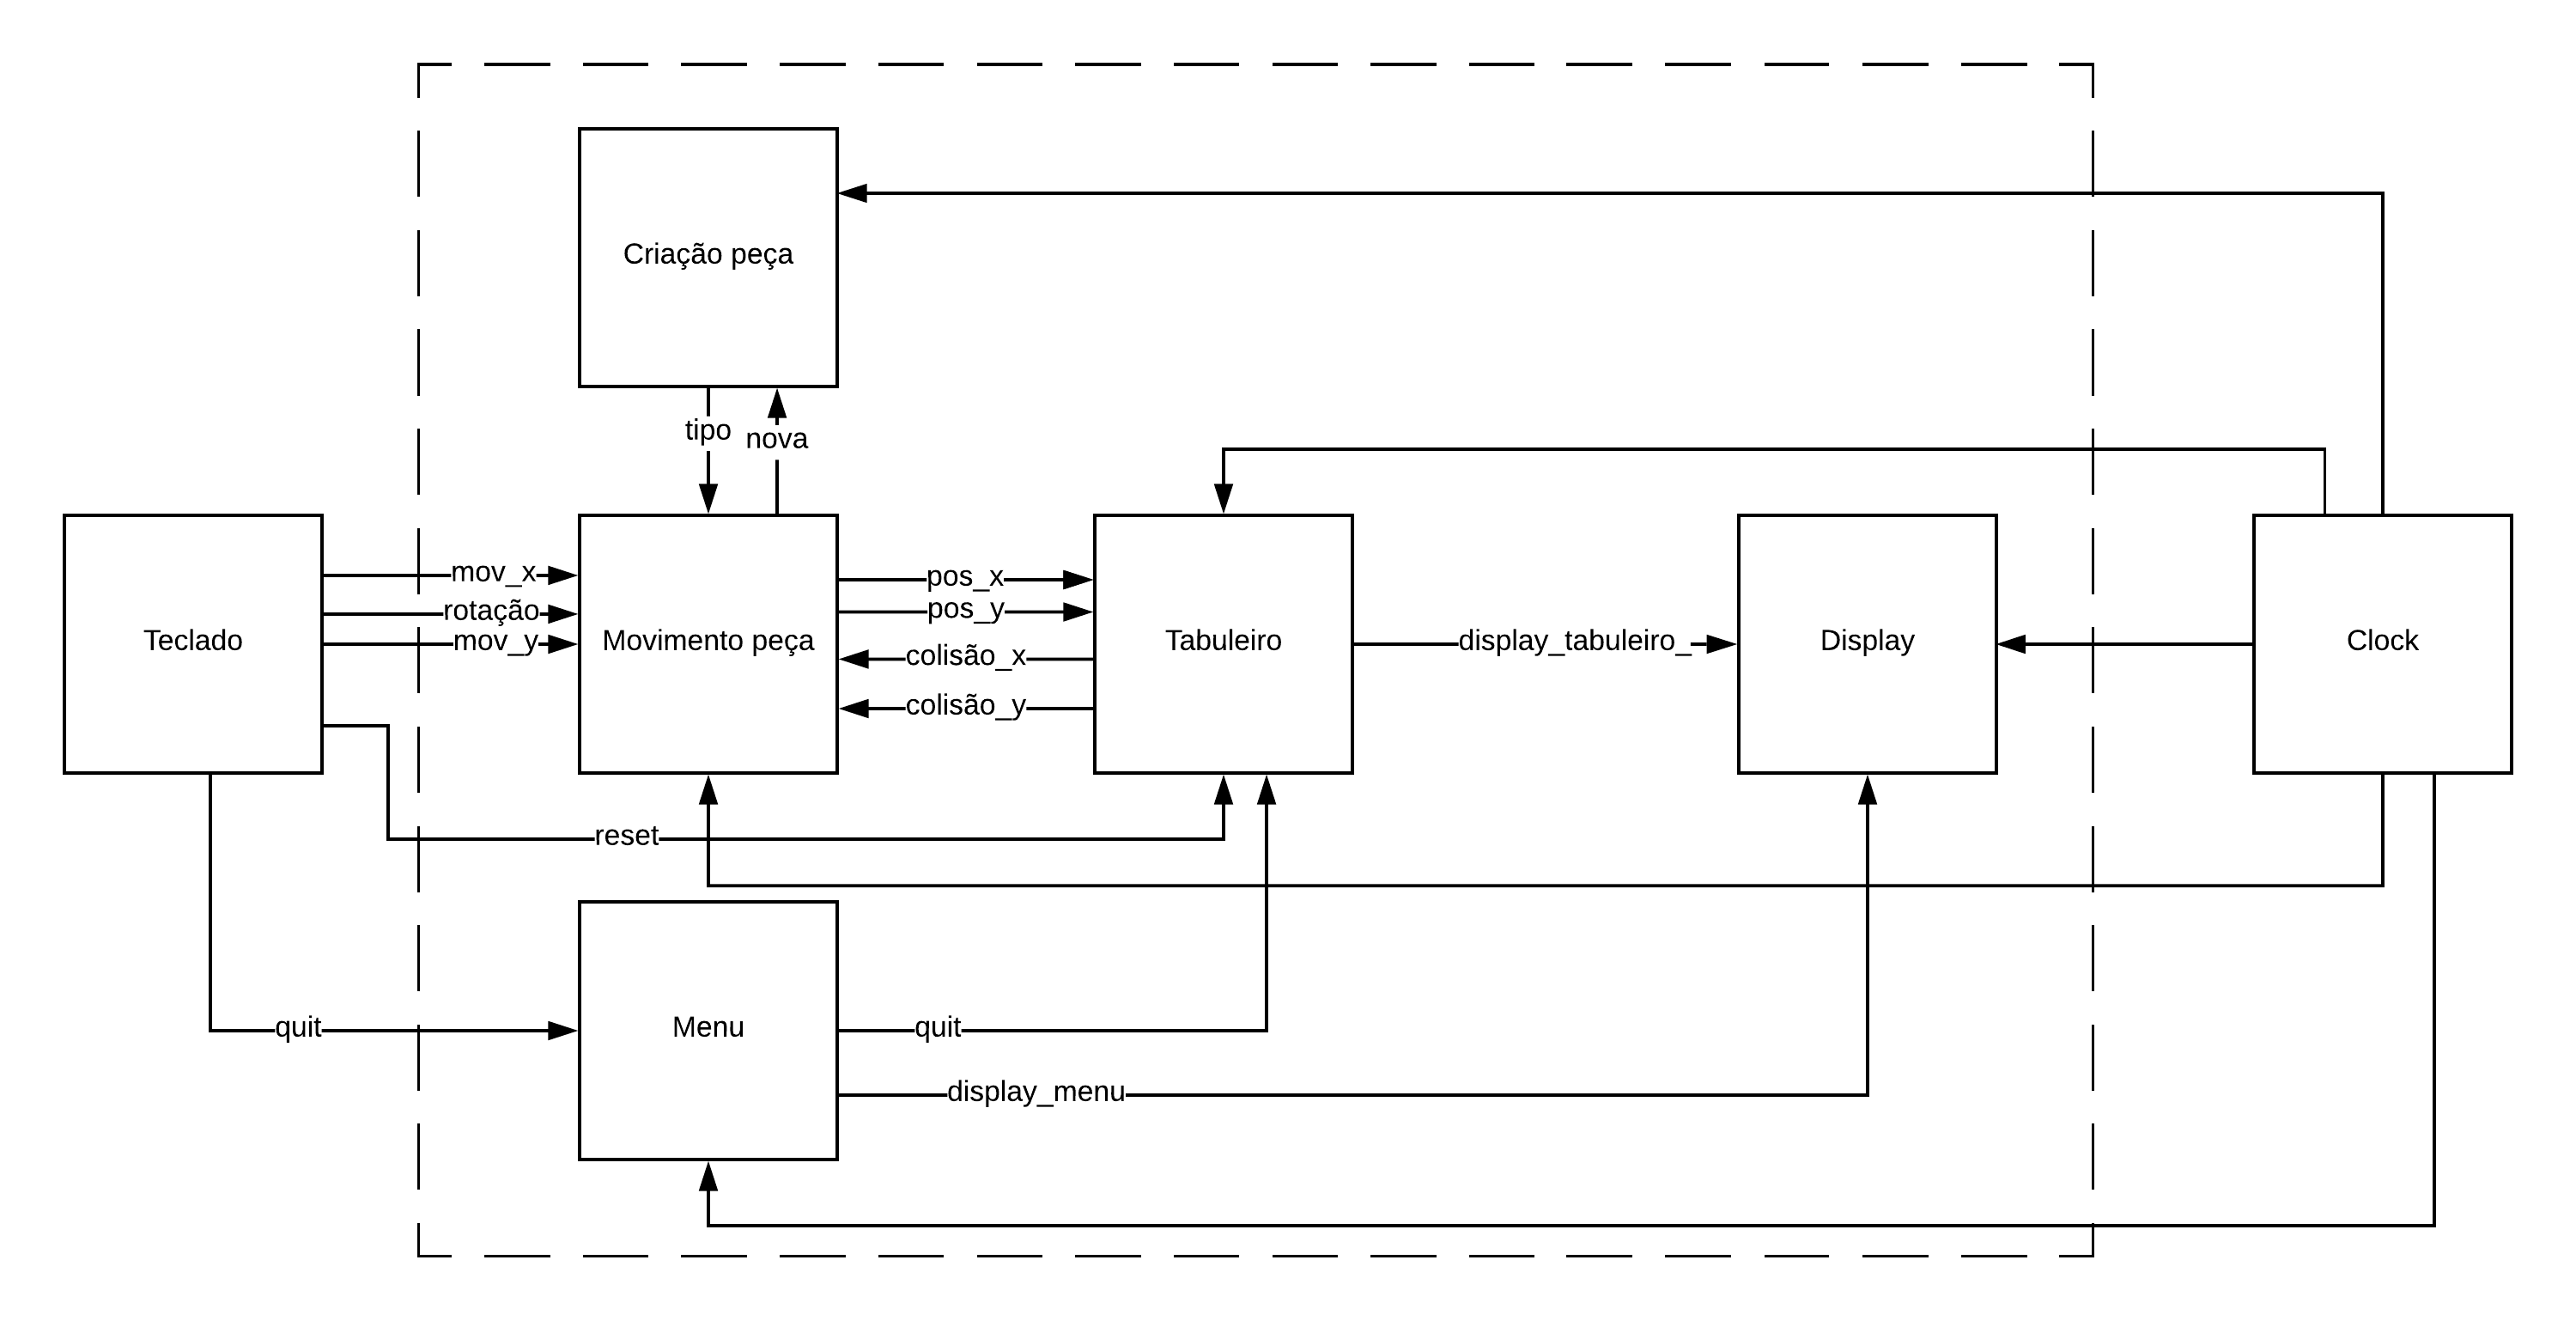
\includegraphics[width=\textwidth]{Diagrama_de_blocos}
\caption{Diagrama de blocos}
\end{figure}

\section{Descri\c{c}\~ao Funcional}
O jogo inicializa no menu de onde pode-se come\c{c}ar um jogo novo. Nesse momento o tabuleiro controla o que aparece no display. Uma pe\c{c}a nova \'e criada e e o componente  movimento pe\c{c} a controla, recebendo a entrada do usu\'ario atrav\'es do teclado. Assim a cada clock o display \'e atualizado de acordo com o tabuleiro e o movimento da pe\c{c}a.

\subsection{Teclado}
Este recebe a entrada do usu\'ario, \'e um componente externo utilizado para o controle das pe\c{c}as, iniciar e reiniciar o jogo. 

\subsection{Menu}
O menu \'e a tela inicial e a tela que aparece após o usuario apertar o botão de quit. Desde ela se pode come\c{c}ar um novo jogo.

\subsection{Tabuleiro}
O tabuleiro controla a l\'ogica principal do jogo, salva a posi\c{c}ao das pe\c{c}as, trata a colis\~ao com a pe\c{c}a atual e a pontua\c{c}\~ao do jogador. 

\subsection{Movimento Pe\c{c}a}
Este componente trata o movimento da pe\c{a} atual. Recebe o tipo de pe\c{c}a do componente Cria\c{c}\~ao de Pe\c{c}a. Controla o movimento e rota\c{c}\~ao de acordo com o recebido do teclado. Envia as informa\c{c}oes para o tabuleiro e recebe de volta se foi poss\'ivel realizar o movimento.

\subsection{Cria\c{c}\~ao de pe\c{c}a}
Depois da pe\c{c}a atual ser colocada no tabuleiro ( e tamb\'em no inicio de cada jogo), o componente cria uma nova pe\c{c}a de um dos sete tipos poss\'iveis, e a passa para o  componente Movimento Pe\c{c}a, que faz com que se torne na pe\c{c}a atual.

\subsection{Display}
Este componente trata da exibi\c{c}\~ao do jogo. Ele recebe informa\c{c}\~oes dos componentes Tabuleiro e Movimento Pe\c{c}a e as exibe na tela.  
\end{document}
